\documentclass[aspectratio=169]{beamer}

\title{Optimizing the Django Admin}
\author{David Fischer (djfische@gmail.com)}
\date{November 21, 2019}

%% Beamer Themes
\usetheme{Berlin}
\usecolortheme{dove}
\usefonttheme{serif}

%% Remove beamer controls
\beamertemplatenavigationsymbolsempty

%% Packages
% Pygments must be accessible to use minted and --shell-escape
%  must be used with pdflatex
\usepackage{minted}
\usepackage{hyperref}
\usepackage{multicol}
\usepackage[font=scriptsize,labelformat=empty]{caption}


\setbeamertemplate{footline}{
  \hspace*{.2cm}
  \scriptsize{
    \insertshorttitle
    \hspace*{50pt}
    \hfill
    \insertframenumber/\inserttotalframenumber
    \hspace*{.2cm}
  }
  \vspace{9pt}
}


\begin{document}

\maketitle


% Fragile is required for syntax highlighting
\begin{frame}[fragile]
\frametitle{Some models (trimmed for brevity)}

\begin{multicols}{2}

{\tiny
\begin{minted}{python}
## blog/models.py

class Category(models.Model):
    name = models.CharField(max_length=255)

class Author(models.Model):
    name = models.CharField(max_length=255)
    status = models.CharField(
        choices=(("staff", "Staff"), ("guest", "Guest")),
        max_length=255,
    )

class Post(models.Model):
    title = models.CharField(max_length=200)
    author = models.ForeignKey(
      Author, 
      on_delete=models.CASCADE,
    )
    categories = models.ManyToManyField(Category)
    body = models.TextField()
    publish_date = models.DateTimeField()

    def __str__(self):
        return f'{self.title} by {self.author}'
\end{minted}
} 

\columnbreak

{\tiny
\begin{minted}{python}
## blog/admin.py

@admin.register(Author)
class AuthorAdmin(admin.ModelAdmin):
    list_display = ("name", "status")
    list_editable = ("status",)


@admin.register(Category)
class CategoryAdmin(admin.ModelAdmin):
    list_display = ("name",)


@admin.register(Post)
class PostAdmin(admin.ModelAdmin):
    list_display = (
      "__str__",
      "post_categories", 
      "publish_date",
    )

    def post_categories(self, obj):
        """Show a combined list of categories for each post"""
        return ", ".join([c.name for c in obj.categories.all()])
\end{minted}
}

\end{multicols}

\end{frame}


\begin{frame}
  \begin{figure}[p]
    \centering
    \fbox{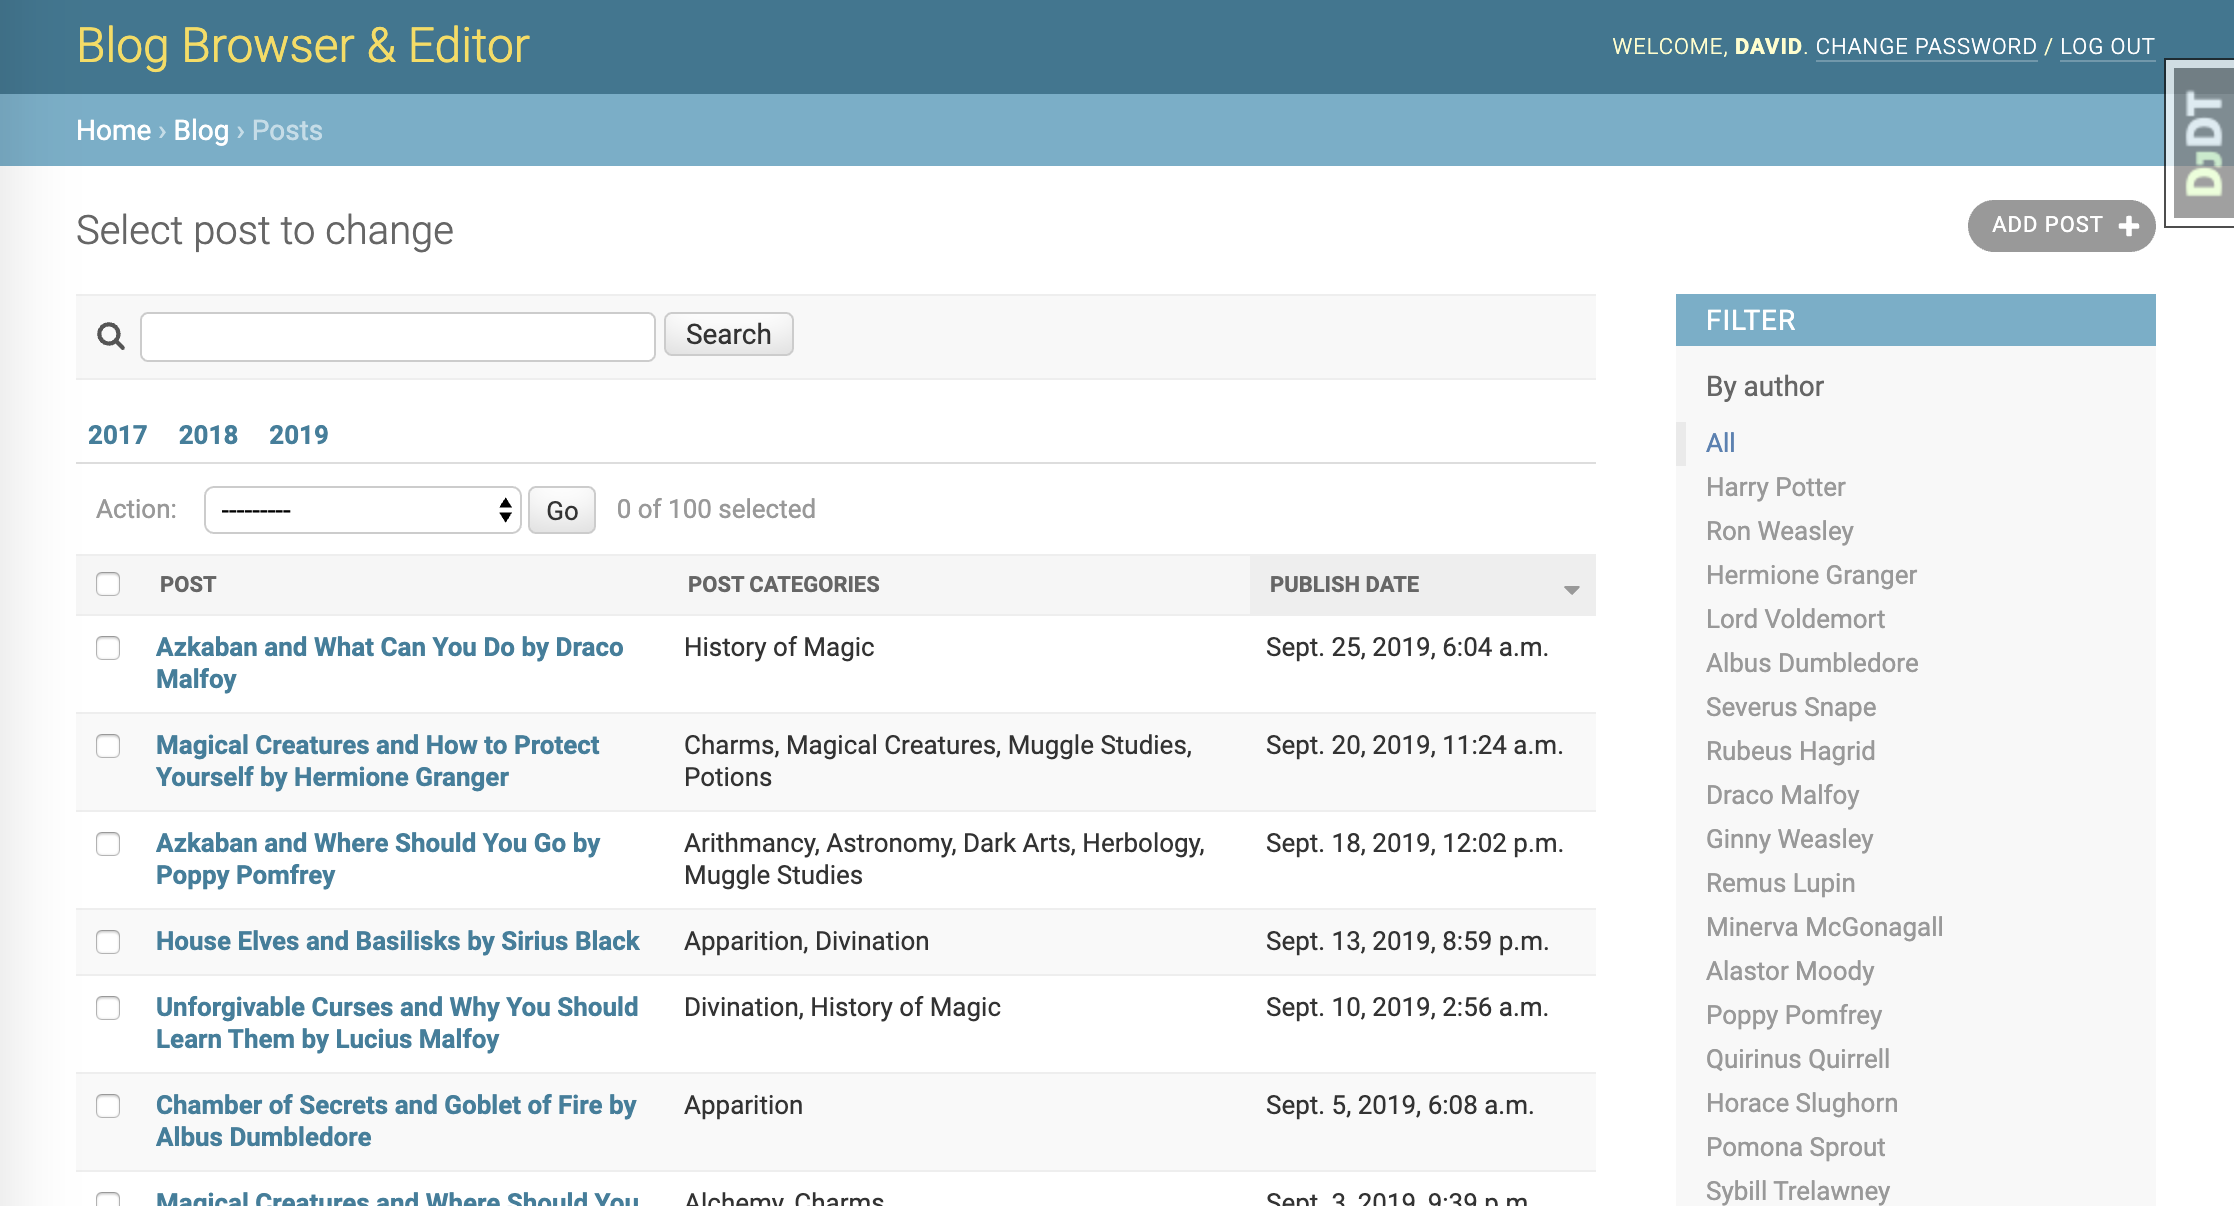
\includegraphics[width=0.8\paperwidth]{images/django-admin-blog.png}}
  \end{figure}
\end{frame}


\begin{frame}
  \begin{figure}[p]
    \centering
    \fbox{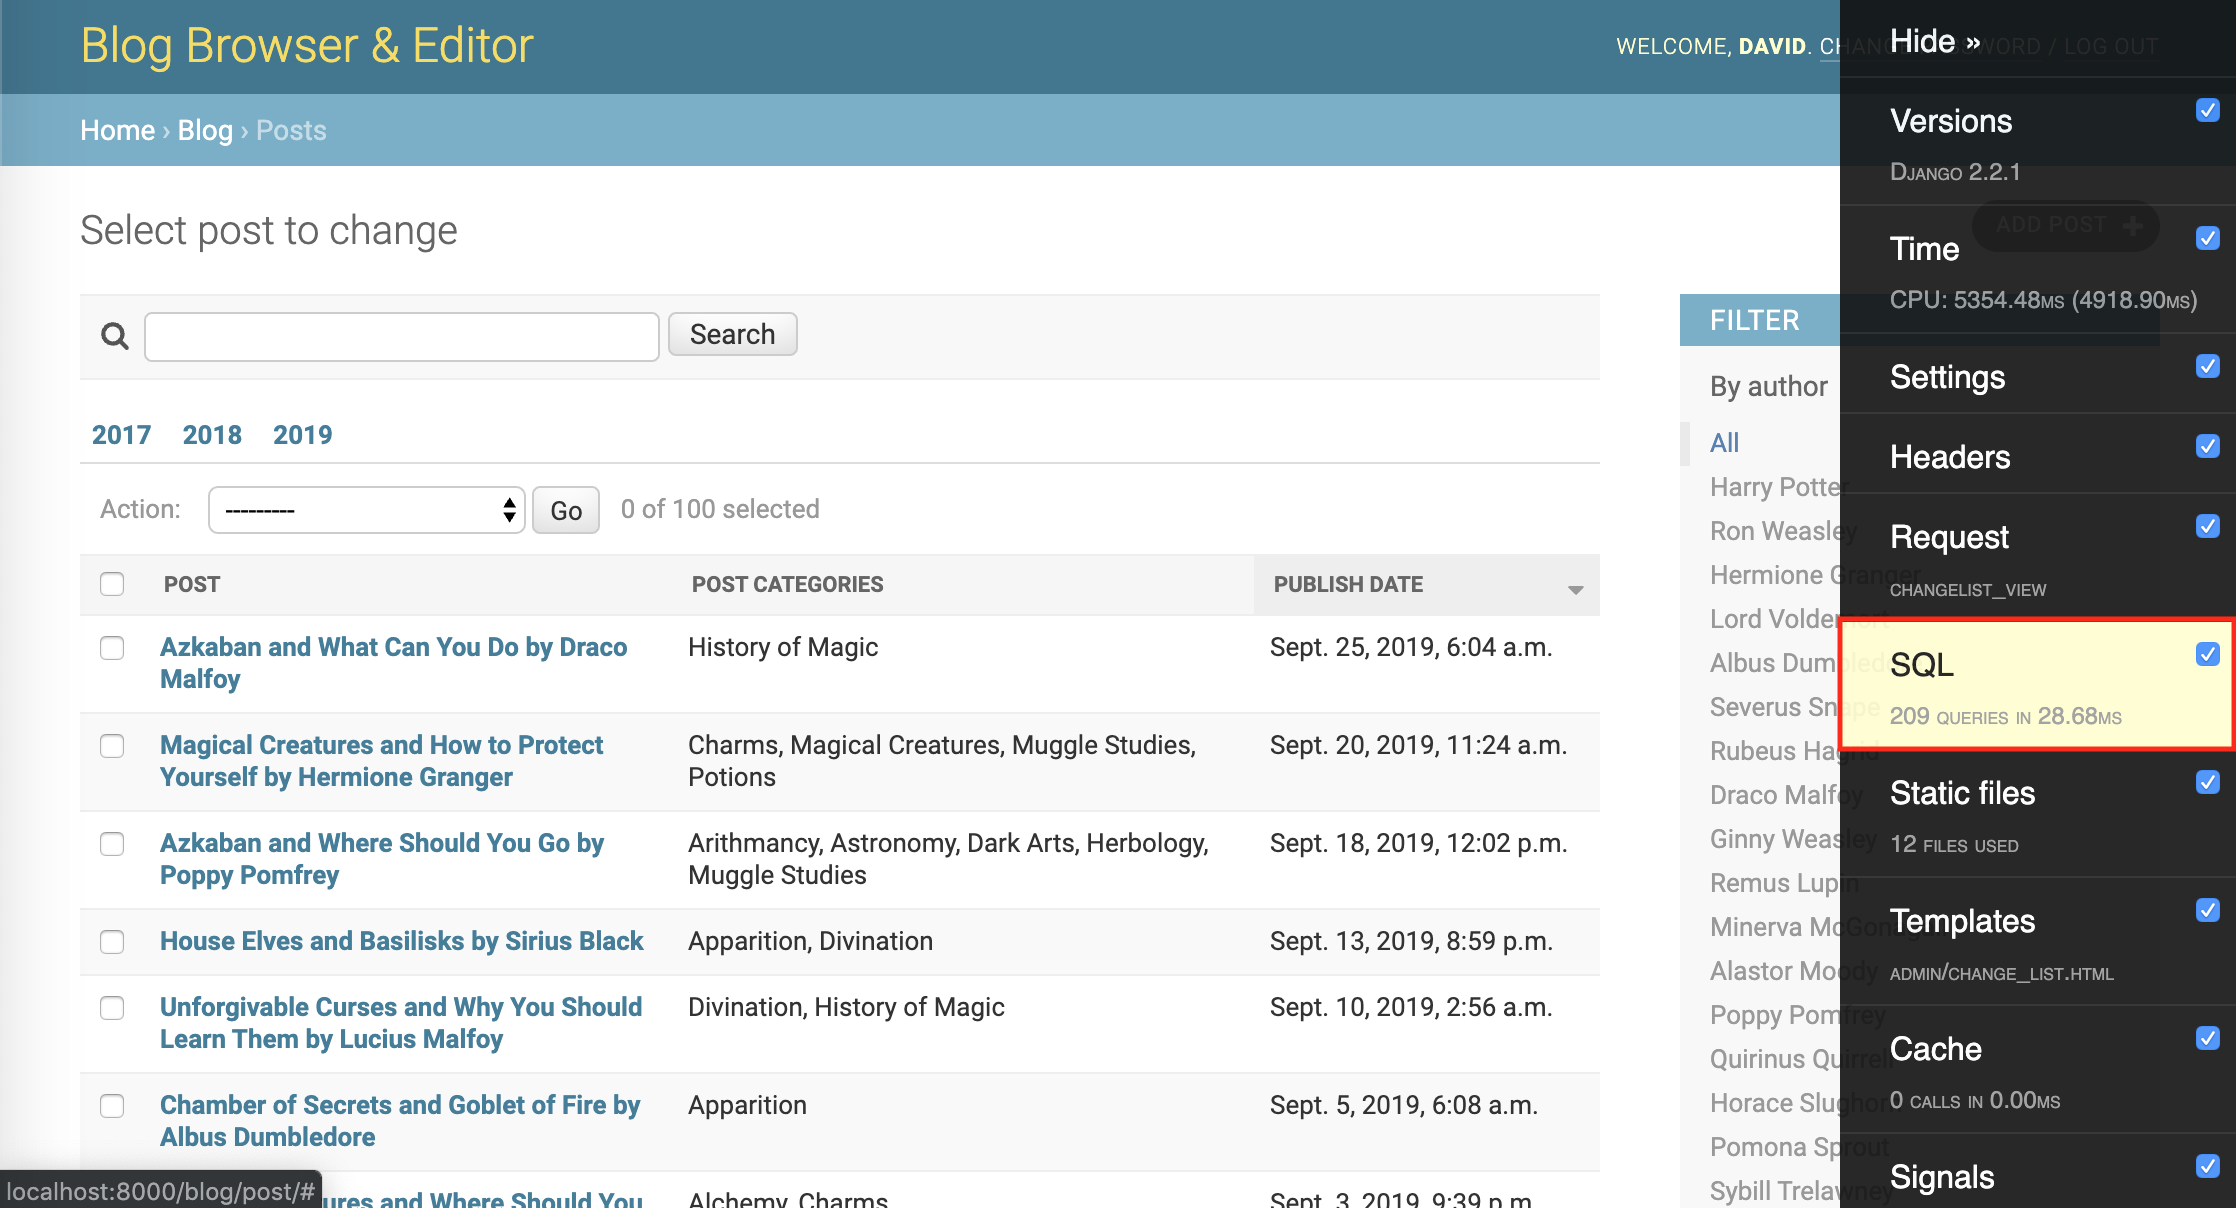
\includegraphics[width=0.8\paperwidth]{images/django-debug-toolbar.png}}
  \end{figure}
\end{frame}


\begin{frame}
  \begin{figure}[p]
    \centering
    \fbox{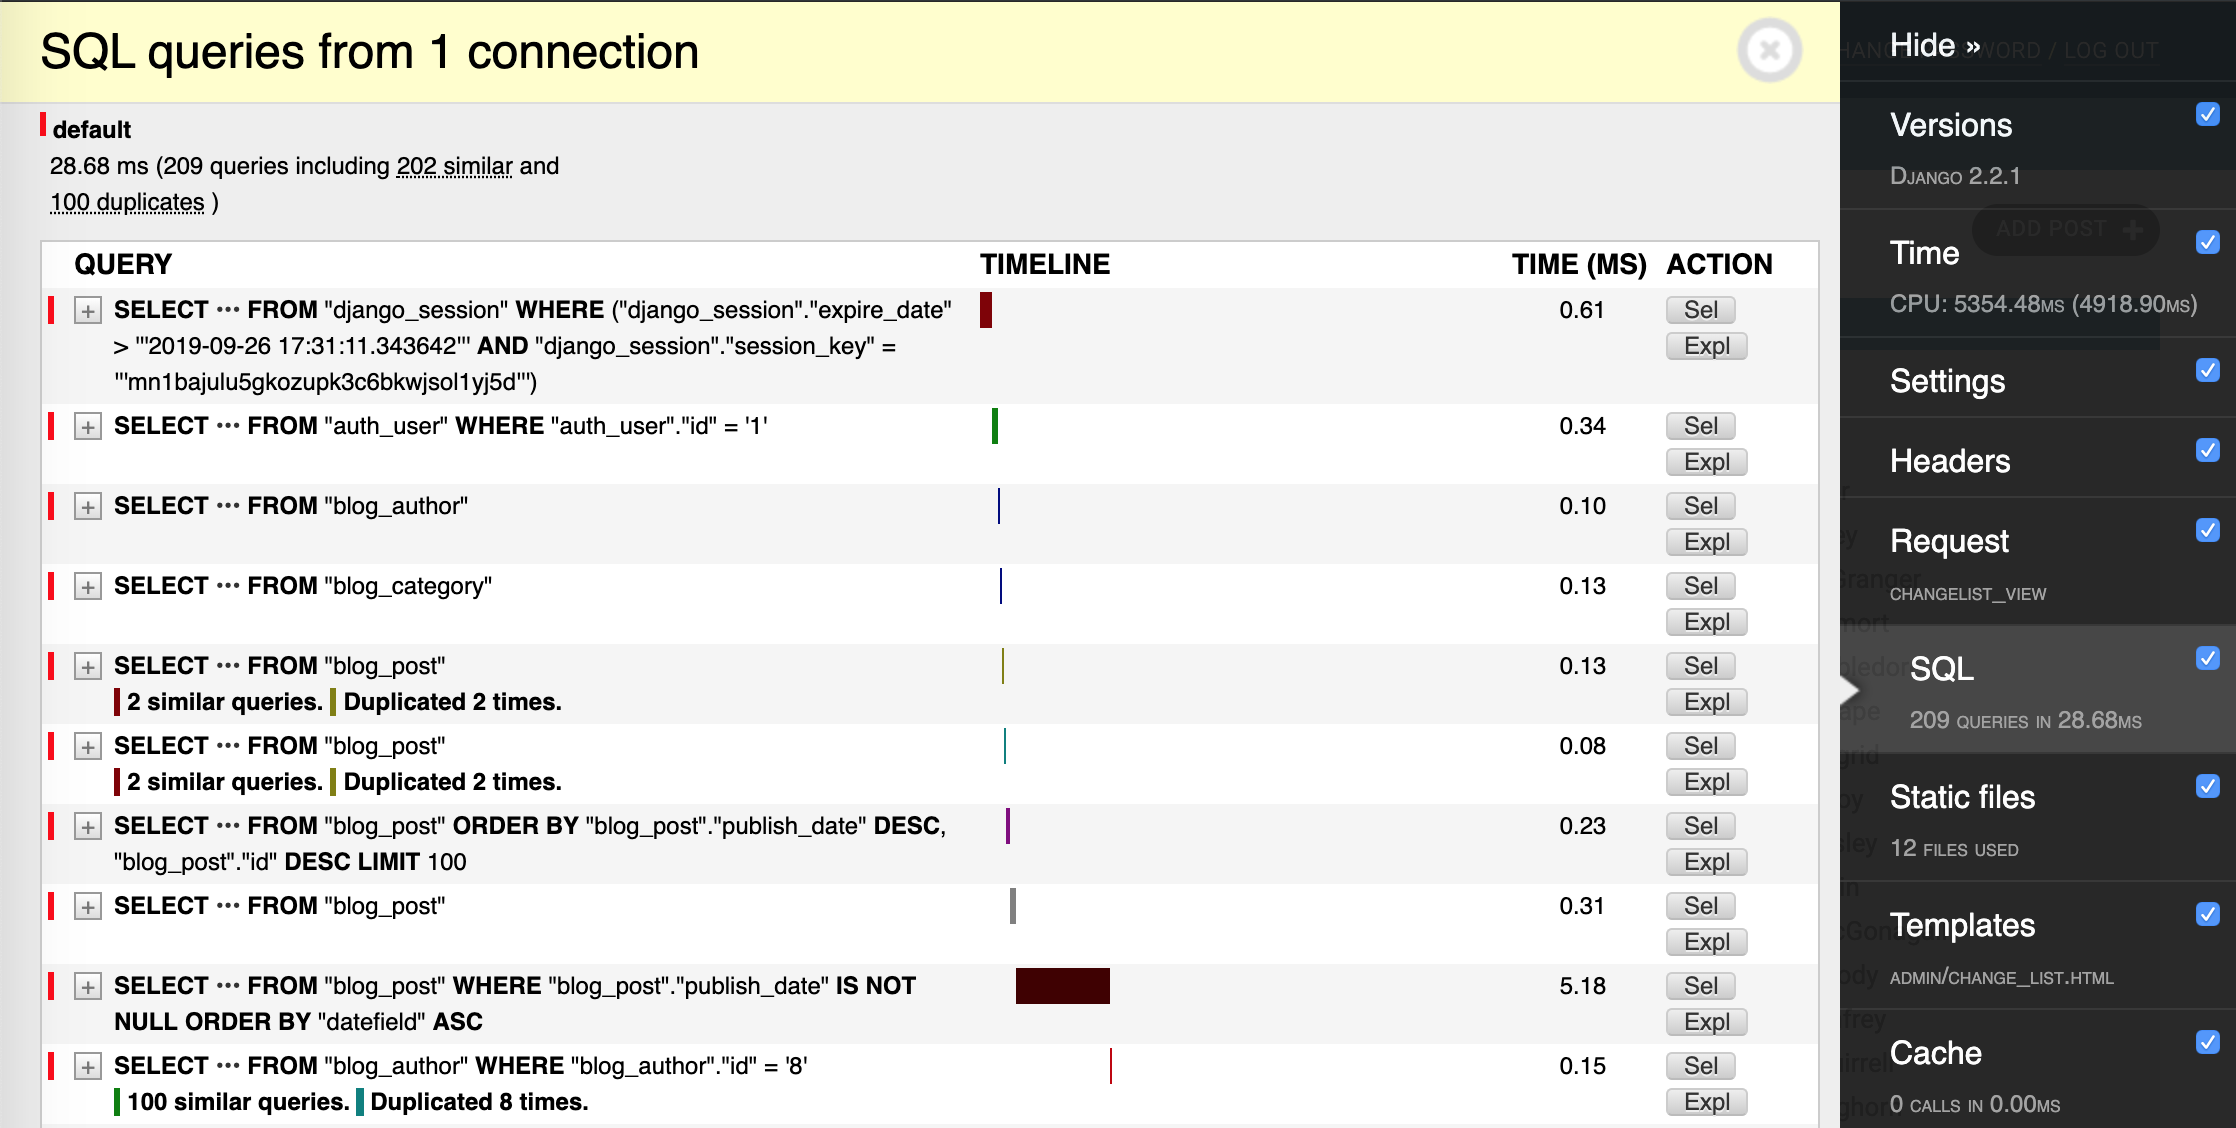
\includegraphics[width=0.8\paperwidth]{images/debug-toolbar-queries.png}}
  \end{figure}
\end{frame}


\begin{frame}[fragile]
\frametitle{One Culprit}

{\tiny
\begin{minted}{python}
## blog/models.py

class Post(models.Model):
    author = models.ForeignKey(Author, on_delete=models.CASCADE)

    # ...

    def __str__(self):
        return f'{self.title} by {self.author}'
\end{minted}
}

\end{frame}


\begin{frame}[fragile]
\frametitle{One Possible Fix}

{\tiny
\begin{minted}{python}
## blog/admin.py

@admin.register(Post)
class PostAdmin(admin.ModelAdmin):
    # ...
    list_select_related = ("author",)
\end{minted}
}

\end{frame}


\begin{frame}[fragile]
\frametitle{Another Possible Fix}

{\tiny
\begin{minted}{python}
## blog/admin.py

@admin.register(Post)
class PostAdmin(admin.ModelAdmin):
    # ...
    list_display = ("title", "author", "post_categories", "publish_date")
\end{minted}
}

\end{frame}


\begin{frame}
  \begin{figure}[p]
    \centering
    \fbox{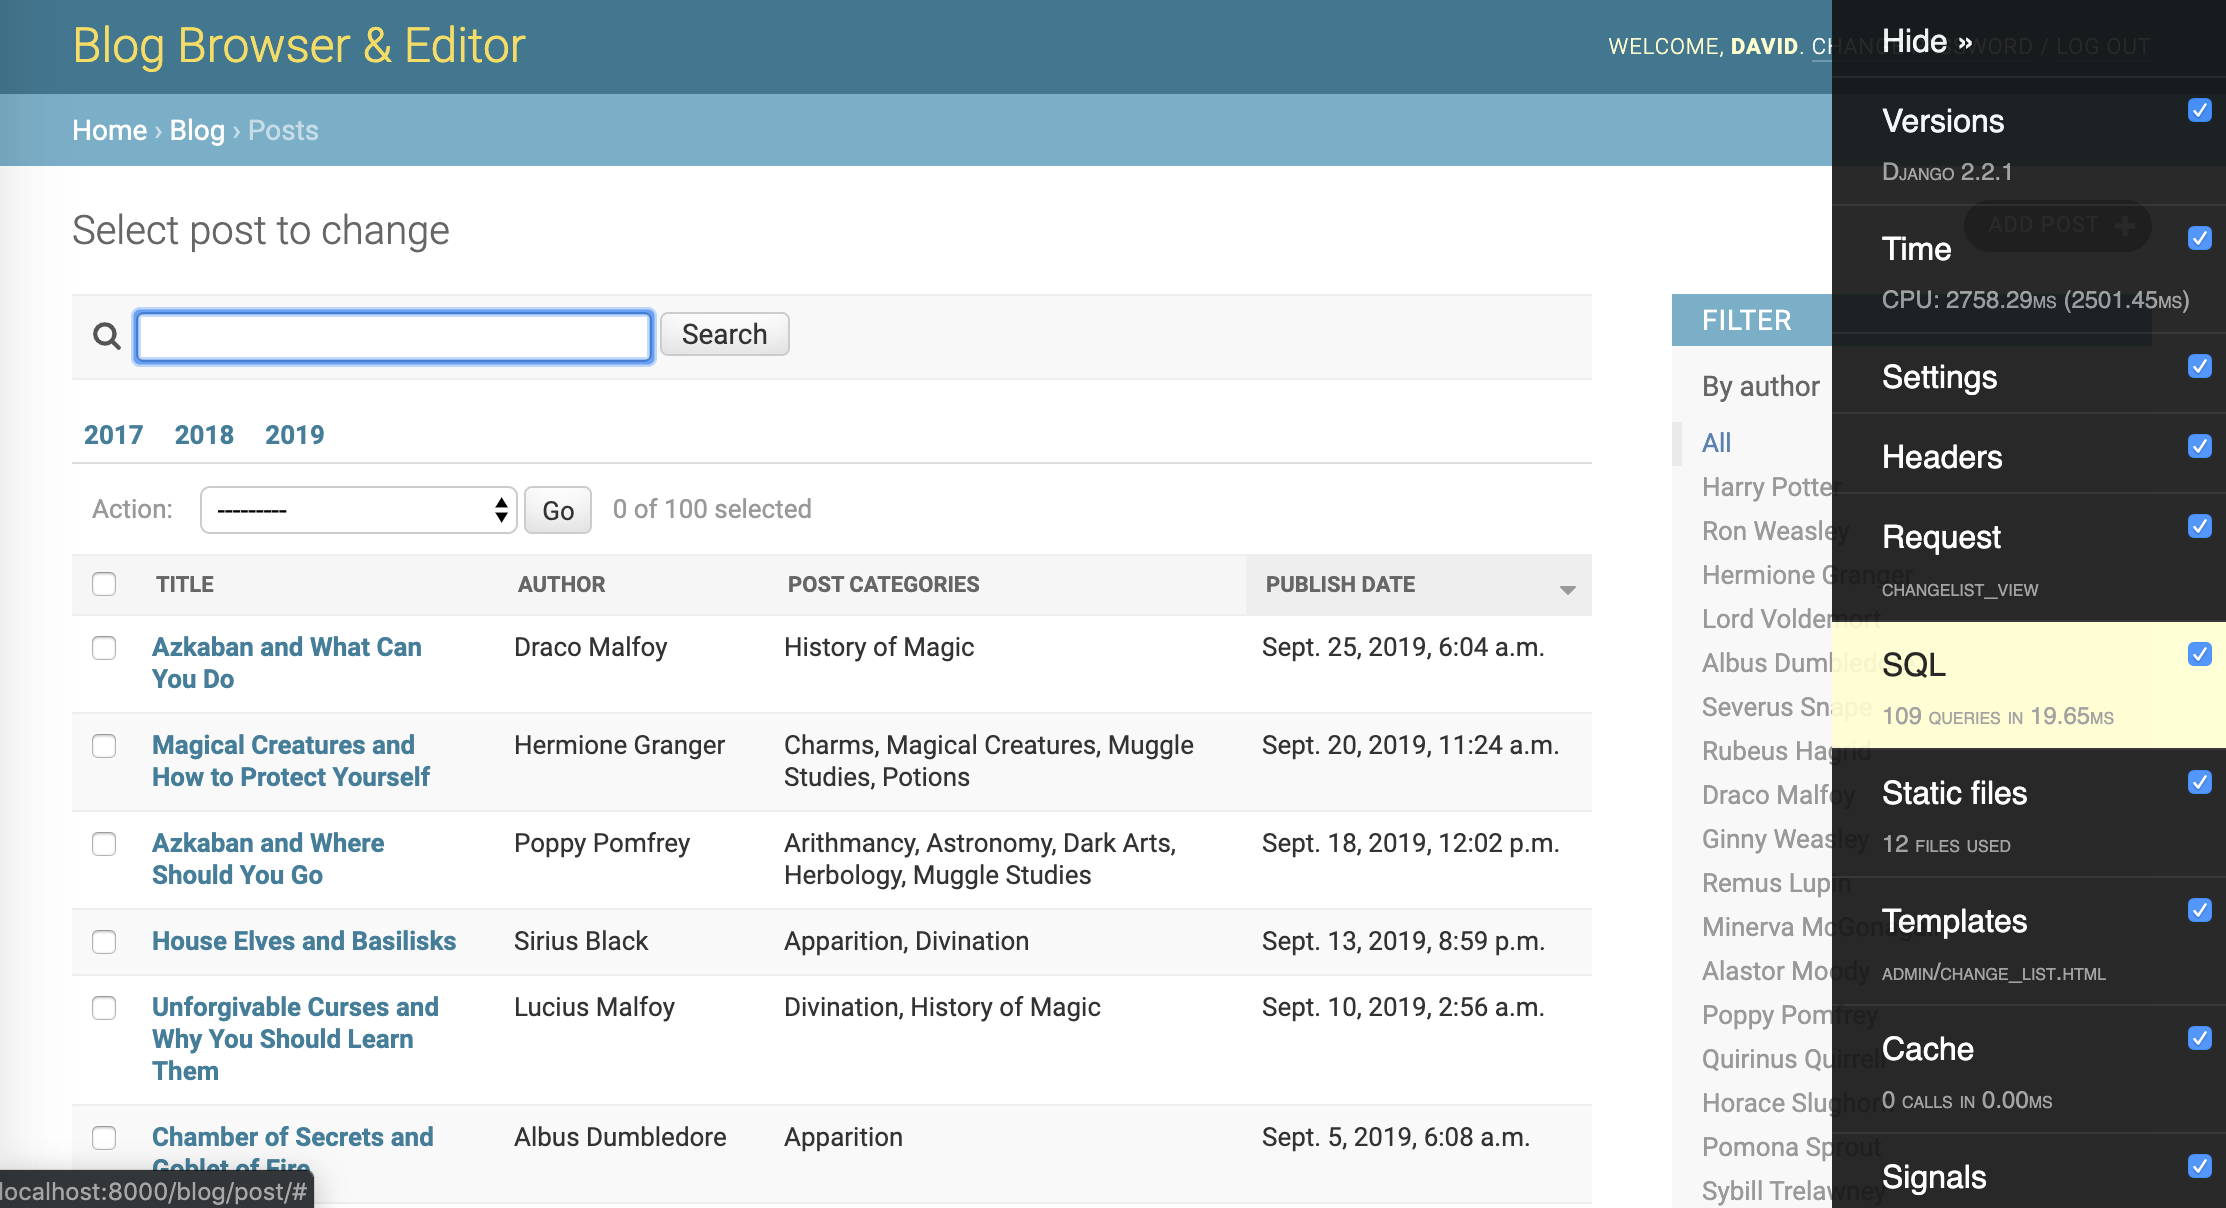
\includegraphics[width=0.8\paperwidth]{images/half-done.png}}
  \end{figure}
\end{frame}


\begin{frame}[fragile]
\frametitle{Another Culprit}

{\tiny
\begin{minted}{python}
## blog/admin.py

@admin.register(Post)
class PostAdmin(admin.ModelAdmin):
    # ...

    def post_categories(self, obj):
        """Show a combined list of categories for each post"""
        return ", ".join([c.name for c in obj.categories.all()])
\end{minted}
}

\end{frame}


\begin{frame}[fragile]
\frametitle{Handling Reverse FK Relations or ManyToMany Relations}

{\tiny
\begin{minted}{python}
## blog/admin.py

@admin.register(Post)
class PostAdmin(admin.ModelAdmin):
    # ...

    def get_queryset(self, request):
        qs = super().get_queryset(request)
        qs = qs.prefetch_related("categories")
        return qs
\end{minted}
}

\end{frame}


\begin{frame}
  \begin{figure}[p]
    \centering
    \fbox{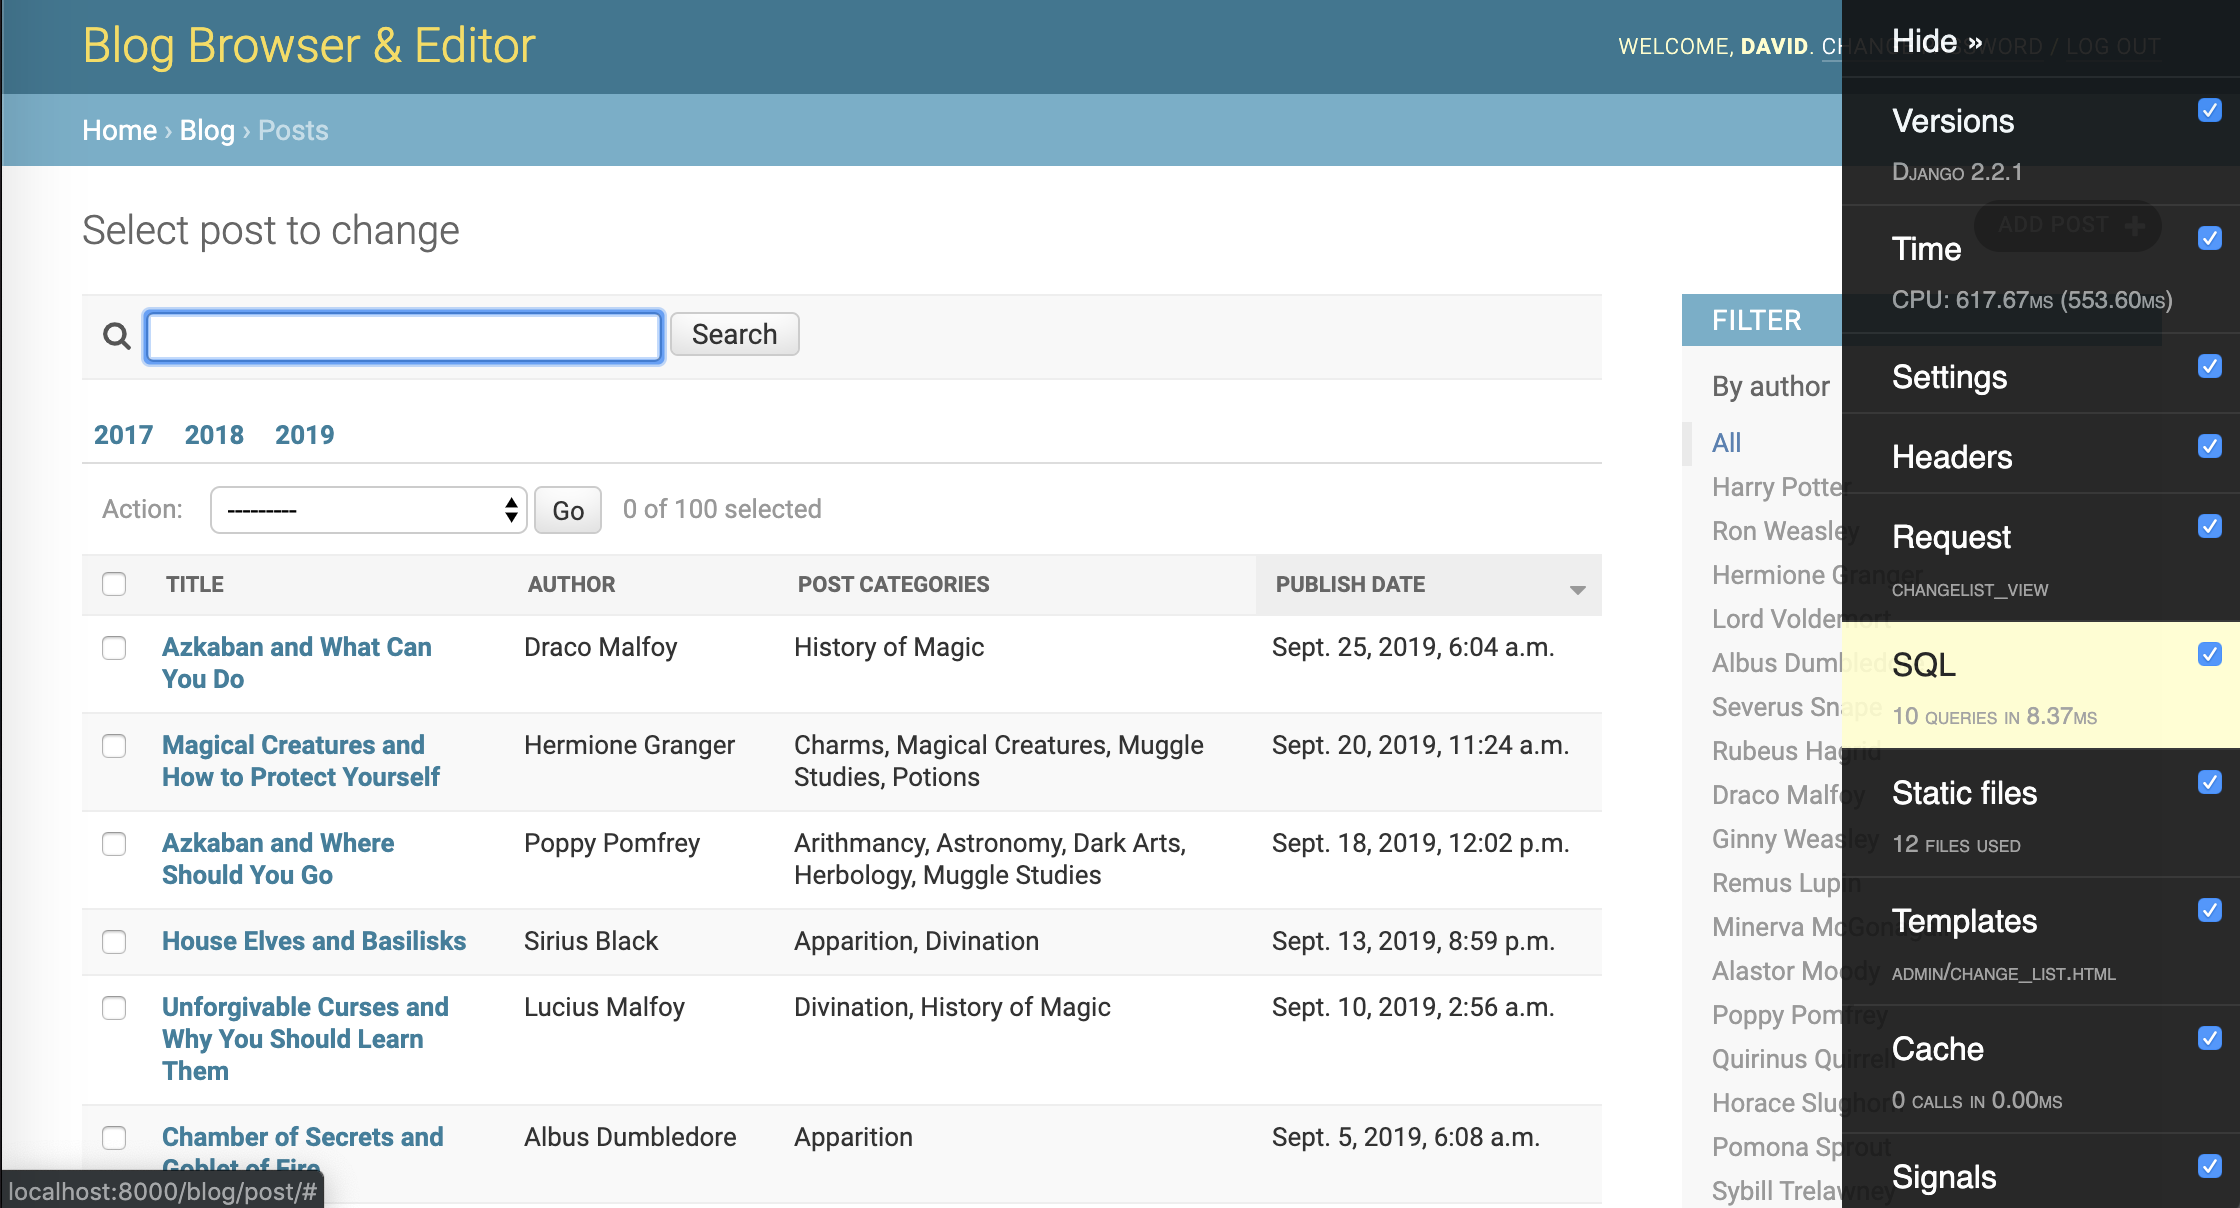
\includegraphics[width=0.8\paperwidth]{images/query-optimization-done.png}}
  \end{figure}
\end{frame}


% \begin{frame}
%   \begin{figure}[p]
%     \centering
%     \fbox{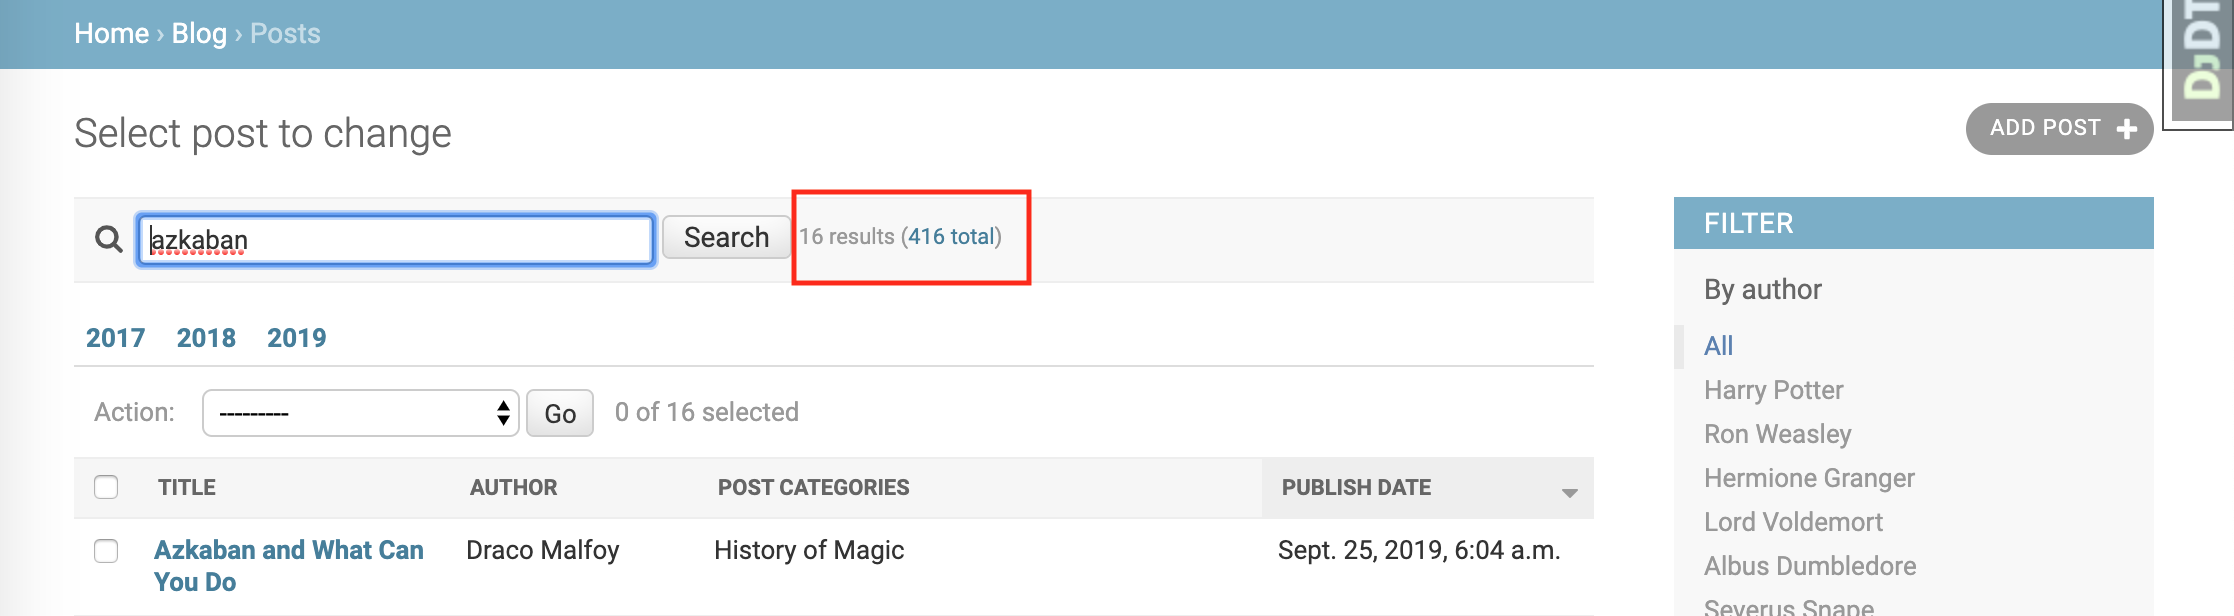
\includegraphics[width=0.8\paperwidth]{images/search-counts.png}}

%     \vfill

%     \fbox{
\includegraphics[width=0.8\paperwidth]{images/pagination.png}}
%   \end{figure}
% \end{frame}


% \begin{frame}[fragile]
% \frametitle{A Partial Fix}
% {\tiny
% \begin{minted}{python}
% ## blog/admin.py

% @admin.register(Post)
% class PostAdmin(admin.ModelAdmin):
%     # ...

%     # Don't show counts on filtered admin pages
%     # (e.g. 99 results (103 total))
%     show_full_result_count = False
% \end{minted}
% }
% \end{frame}


% \begin{frame}[fragile]
% \frametitle{A Fix for Expensive Counts}
% {\tiny
% \begin{minted}{python}
% ## blog/admin.py

% @admin.register(Post)
% class PostAdmin(admin.ModelAdmin):
%     # ...

%     # Use a custom paginator
%     paginator = CustomPaginator
% \end{minted}
% }
% \end{frame}


% \begin{frame}
% \frametitle{Custom Paginator Approaches}
%   \begin{itemize}
%     \item {\small Use a count estimate from your database backend}
%     \item {\small Hard code a large number for the count}
%     \item {\small Cache the number of rows (or otherwise calculate infrequently)}
%   \end{itemize}
% \end{frame}


\begin{frame}
  \begin{figure}[p]
    \centering
    \fbox{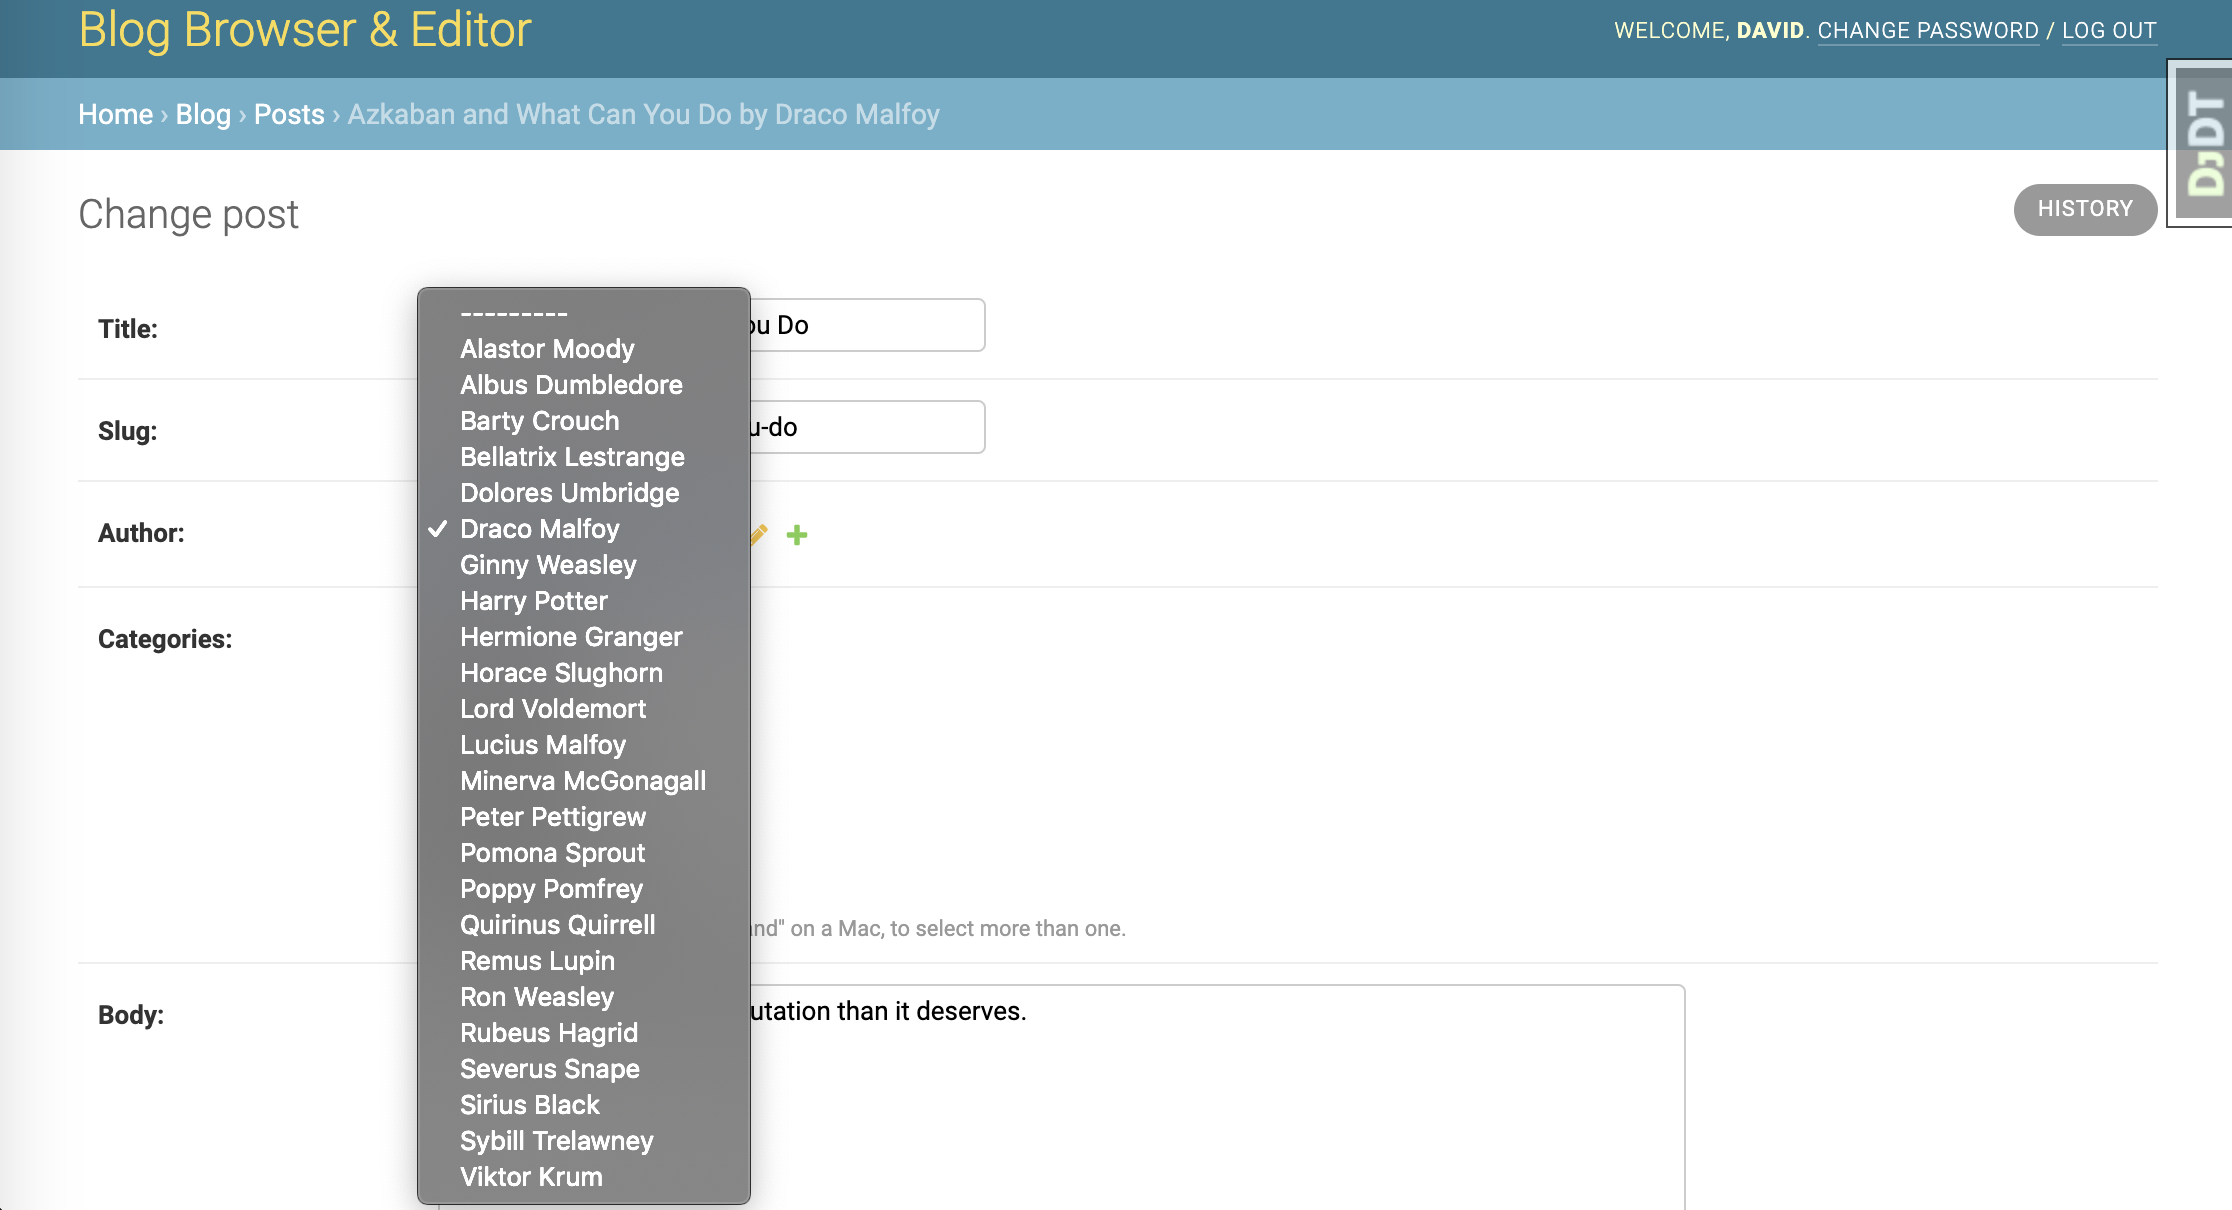
\includegraphics[width=0.8\paperwidth]{images/quantity-foreign-keys.png}}
  \end{figure}
\end{frame}


\begin{frame}[fragile]
\frametitle{Large Numbers of Foreign Key Choices}

{\tiny
\begin{minted}{python}
## blog/admin.py

@admin.register(Post)
class PostAdmin(admin.ModelAdmin):
    # ...

    raw_id_fields = ("author",)
\end{minted}
}

\end{frame}


\begin{frame}
  \begin{figure}[p]
    \centering
    \fbox{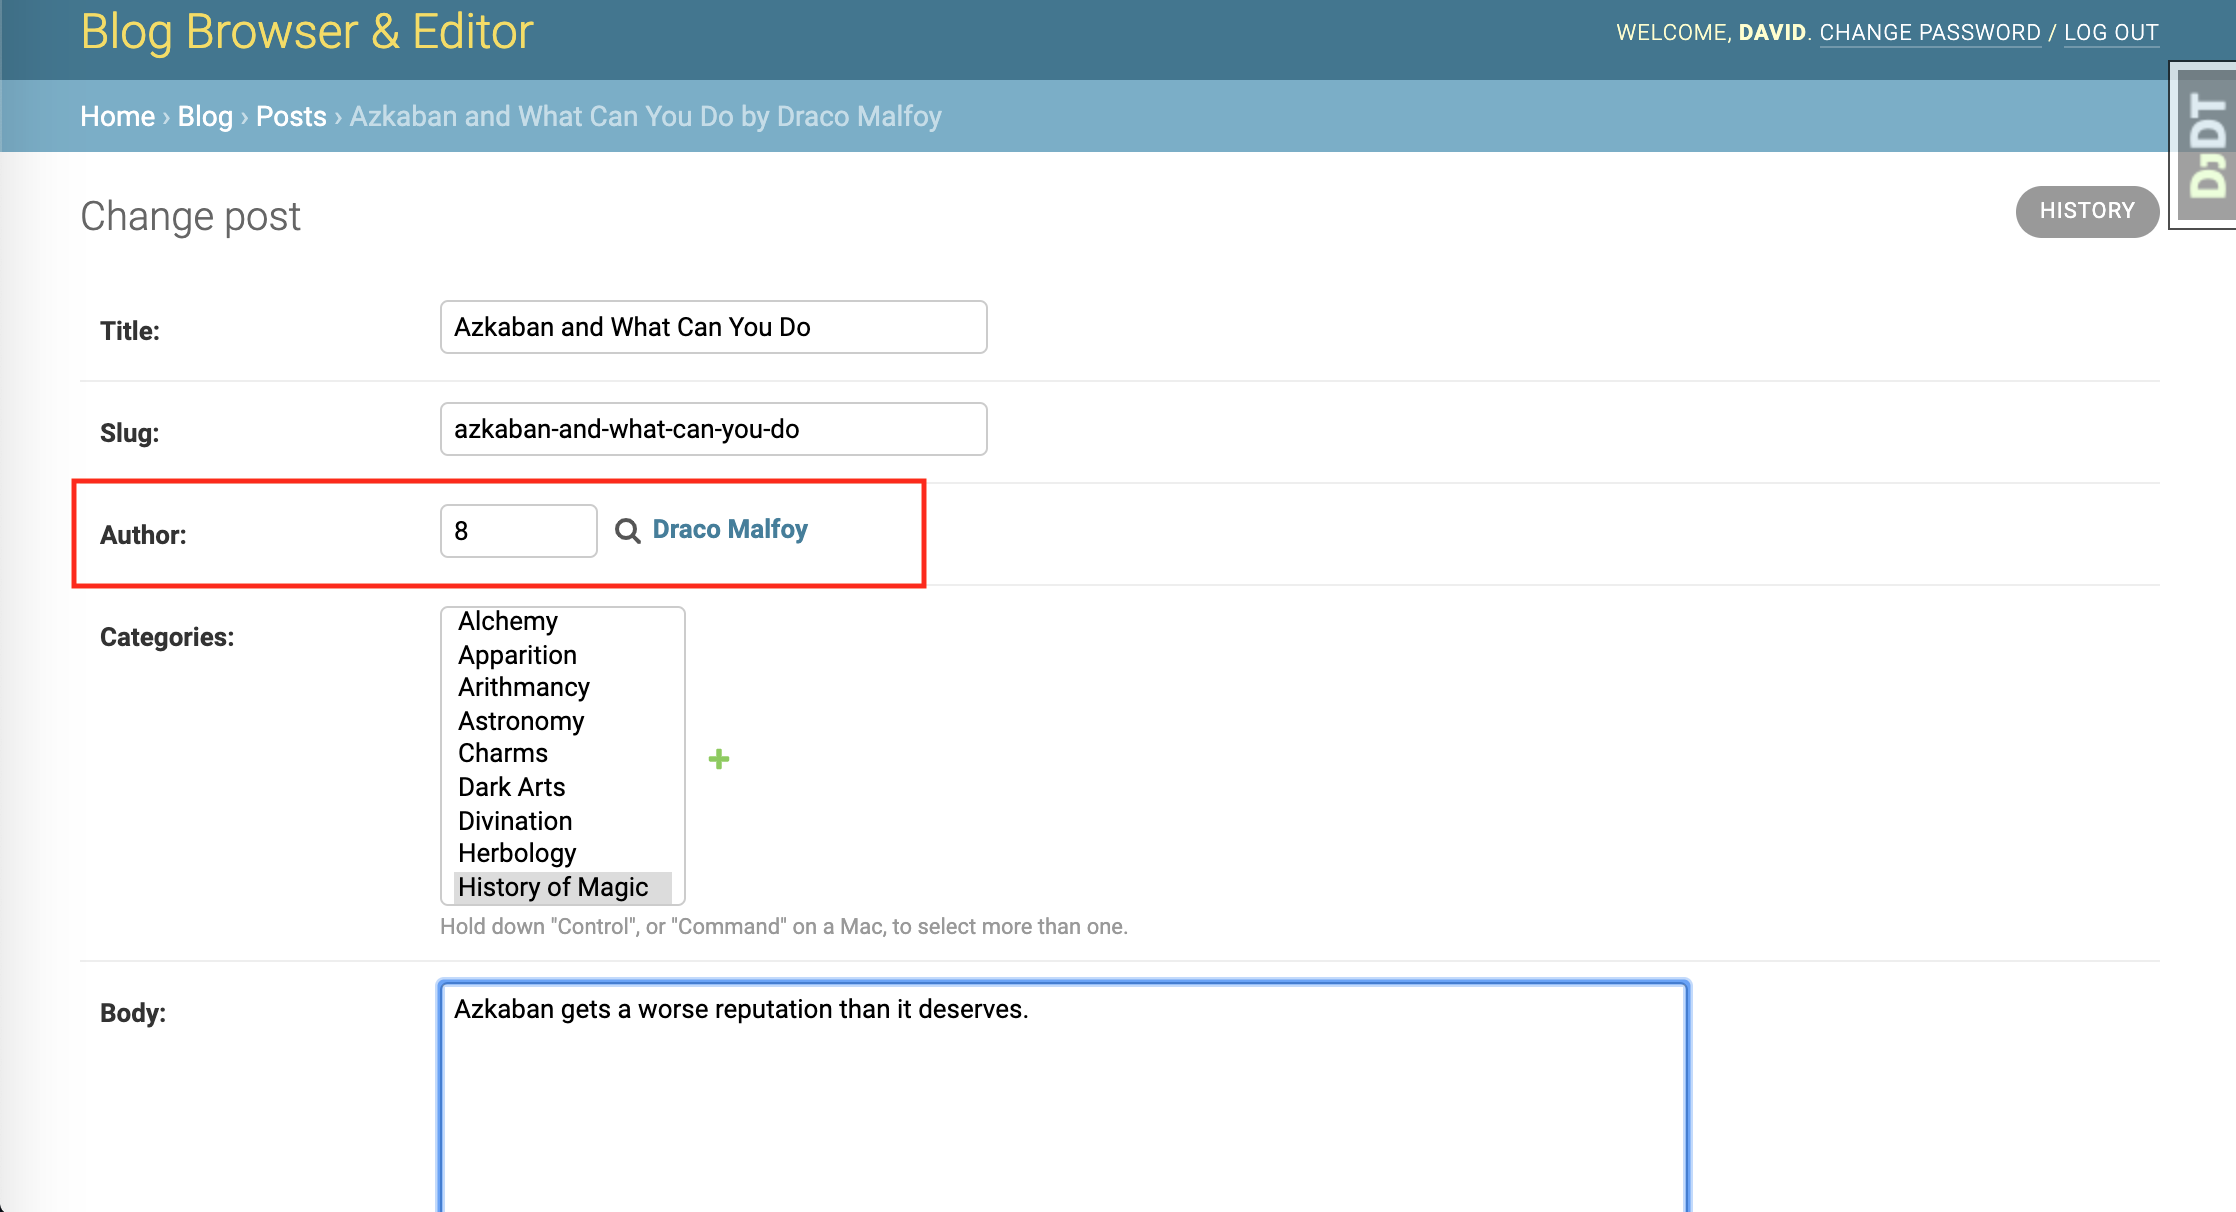
\includegraphics[width=0.8\paperwidth]{images/foreign-key-selector.png}}
  \end{figure}
\end{frame}


\begin{frame}
\frametitle{Resources}
  \begin{itemize}
    \item {\small \href{https://www.youtube.com/watch?v=f8cFjiyxQuQ}{But, Why is the Django Admin Slow? (Jacinda Shelly - PyCon 2019)}}
    \item {\small \href{https://django-debug-toolbar.readthedocs.io/en/latest/}{Django Debug Toolbar}}
    \item {\small \href{https://docs.djangoproject.com/en/2.2/ref/contrib/admin/}{Django Admin Site Docs}}
    \item {\small \href{https://docs.djangoproject.com/en/2.2/topics/db/optimization/}{Django DB Access Optimization Docs}}
    \item {\small Django Admin Cookbook - \href{https://books.agiliq.com/projects/django-admin-cookbook}{books.agiliq.com}}
    \item {\small \href{https://hakibenita.com/tag/django-admin}{hakibenita.com}}
  \end{itemize}
\end{frame}


\begin{frame}
\frametitle{Interested in more Django Admin talks?}
  Past Talks
  \begin{itemize}
    \item {\small \href{https://github.com/davidfischer/talk-customizing-django-admin}{Customizing the Django Admin}}
  \end{itemize}

  \vfill

  Future Talks
  \begin{itemize}
    \item {\small Securing the Django Admin}
    \item {\small Django Admin Add-Ons \& Extensions}
  \end{itemize}
\end{frame}


\begin{frame}
\frametitle{}
  {\huge Questions or comments?}
\end{frame}


\end{document}
